We will now discuss the model-aware optimization of Dolinar-like receivers, which is based in the observations outlined previously regarding the sequential structure of such receivers.

As introduced in Sec.~\ref{ssec:1_rl_dp}, dynammic programming exploits the so-called principle of optimality, which links optimal actions to optimal state value functions through the optimal Bellman equation, see Eq.~\ref{eq:vBellOp}. In there, we introduced Markov Decision Problems (MDP) consisting on an agent that sequentially interacts with its environment in order to maximize a figure of merit known as the return. This quantity captures the amount of rewards the agent collects during an episode, and it here translates to the correcteness of agent's guess, which is obtained after measuring the state by a Dolinar-like receiver. In the MDP section, we have also made the distinction between agent and environment states, which arises due to the impossibility of the agent to have fully access to the environment's state at a given step, and thus Partially Observable Markov Decision Processes were introduced. Here, we will define the environment states as the underlying quantum states $\ket{\alpha_k}$ to be discriminated.

\begin{figure}[t!]
    \centering
    \begin{subfigure}[b]{0.49\textwidth}
        \centering
        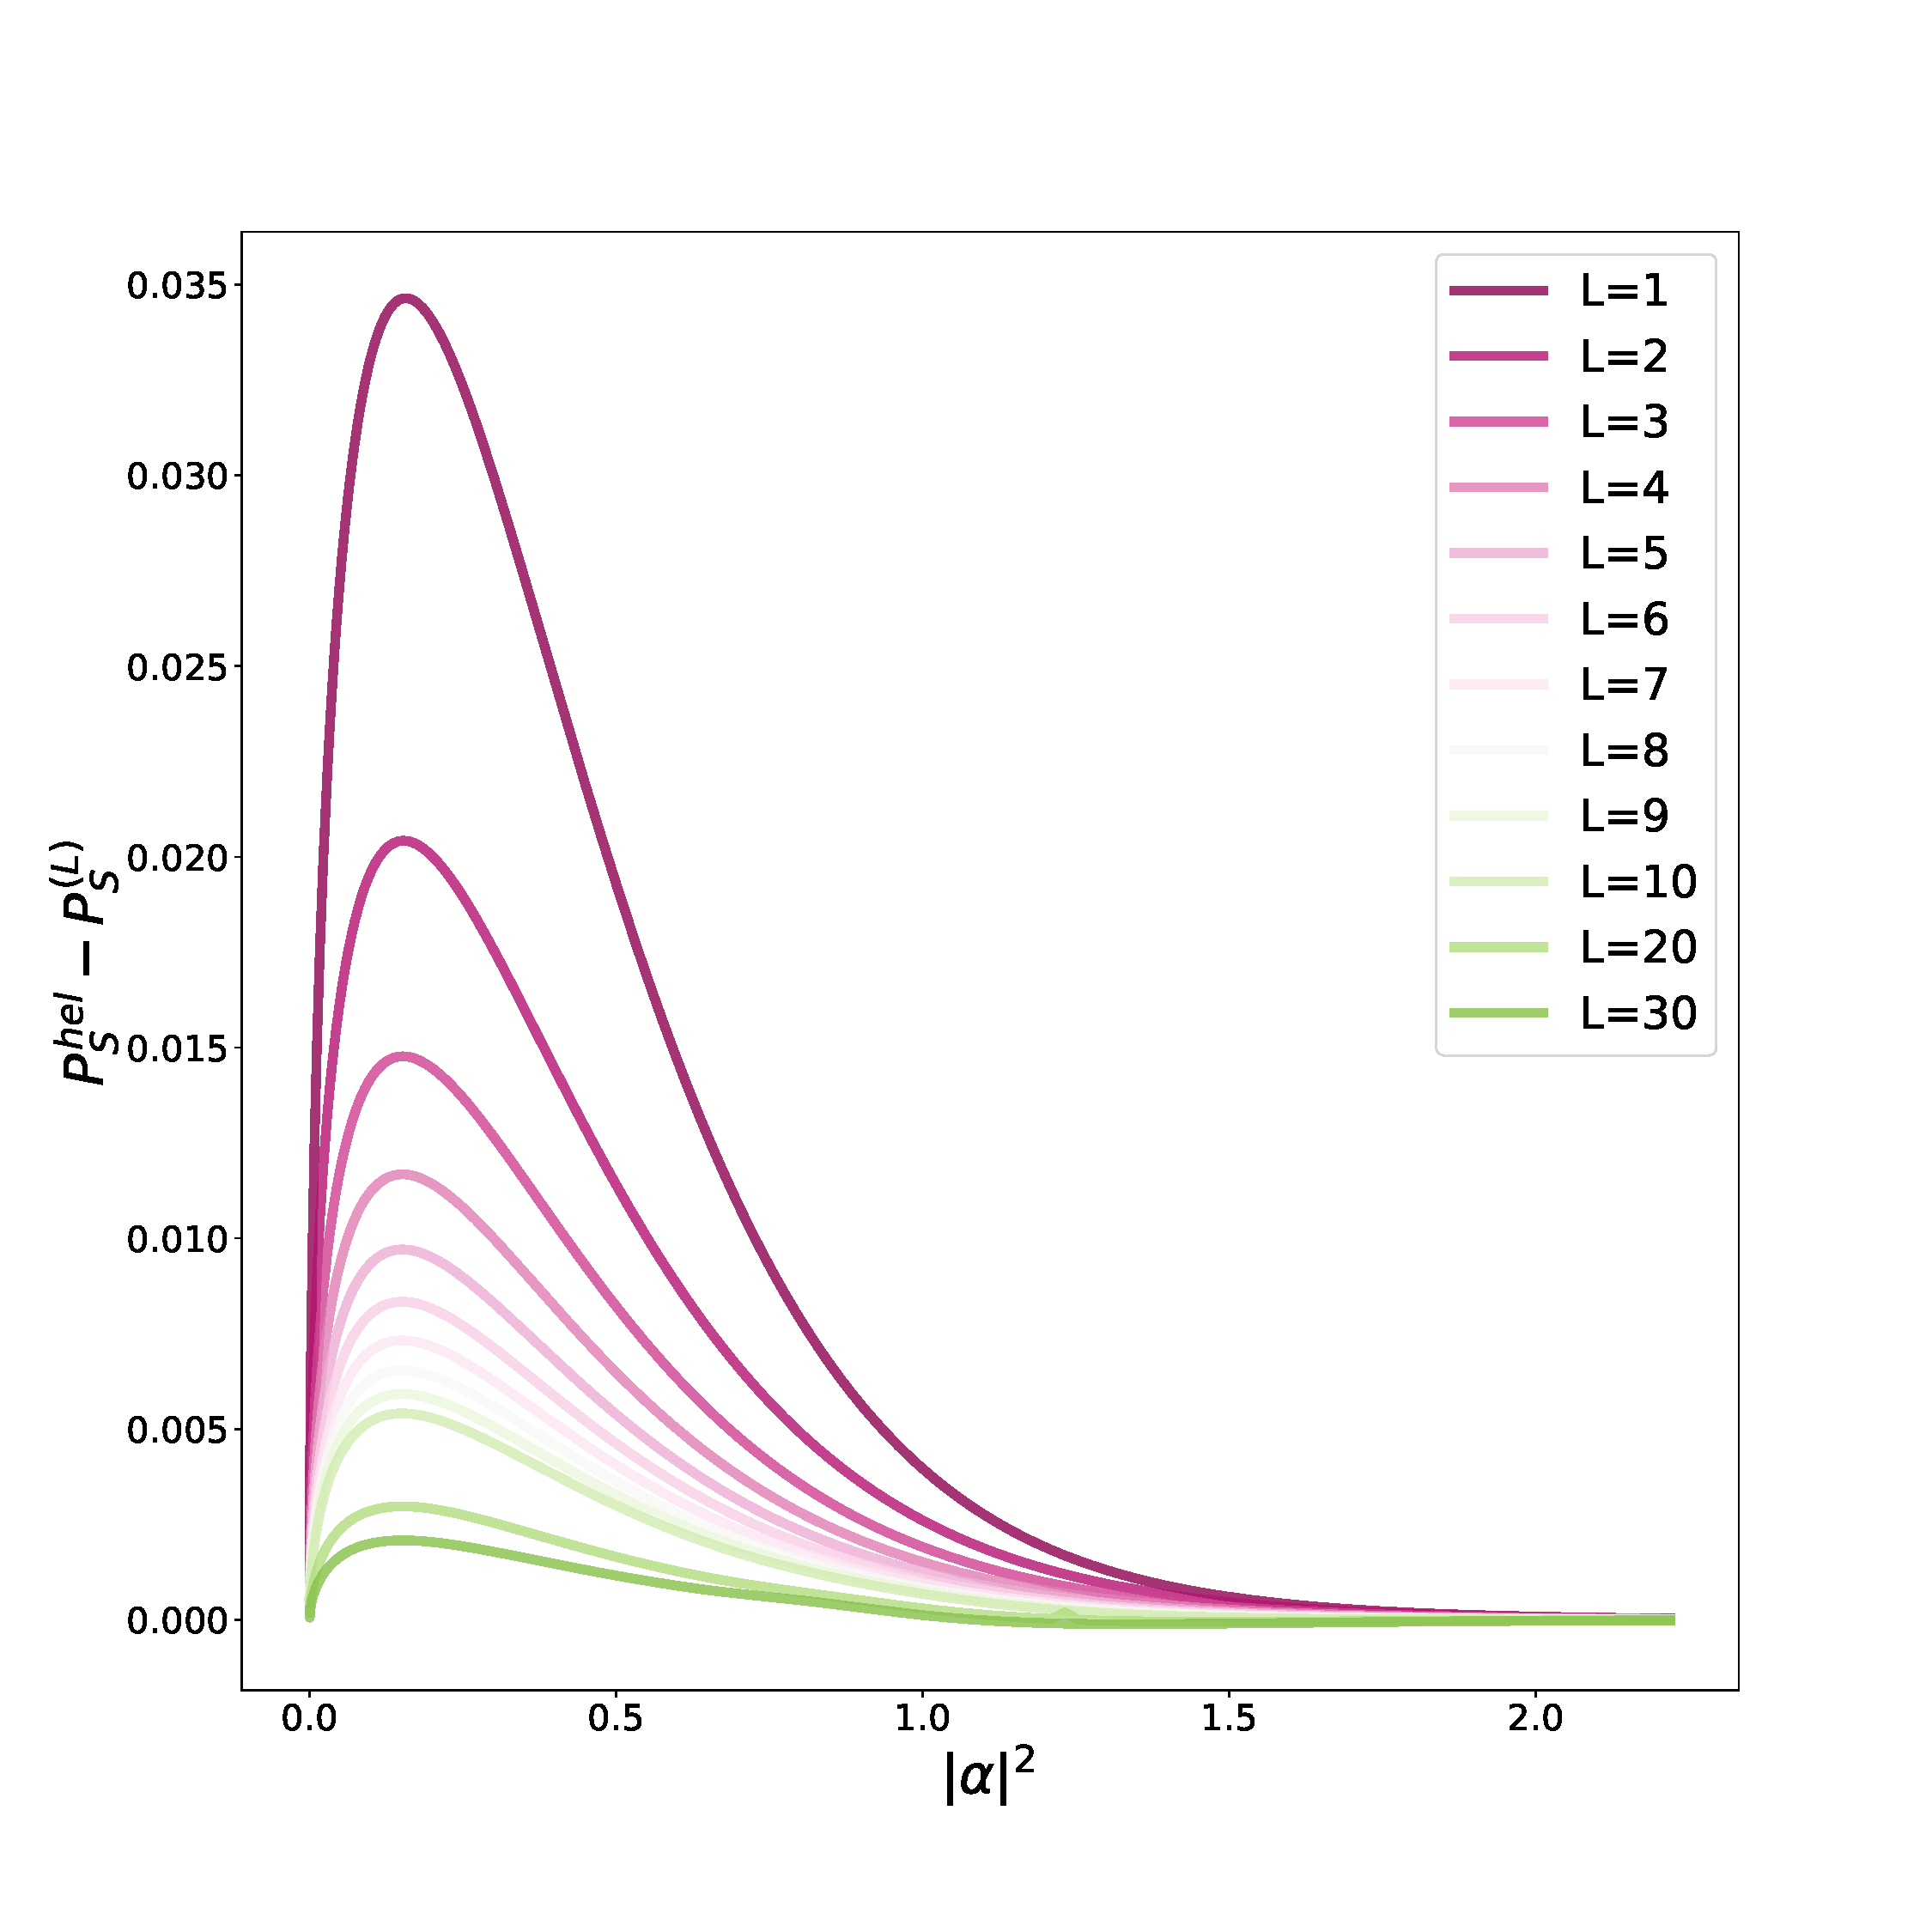
\includegraphics[width=1.\textwidth]{Figures/314/34_dp_results.pdf}
        \caption{}
        \label{fig:dpre1}
    \end{subfigure}
    \begin{subfigure}[b]{0.49\textwidth}
        \centering
        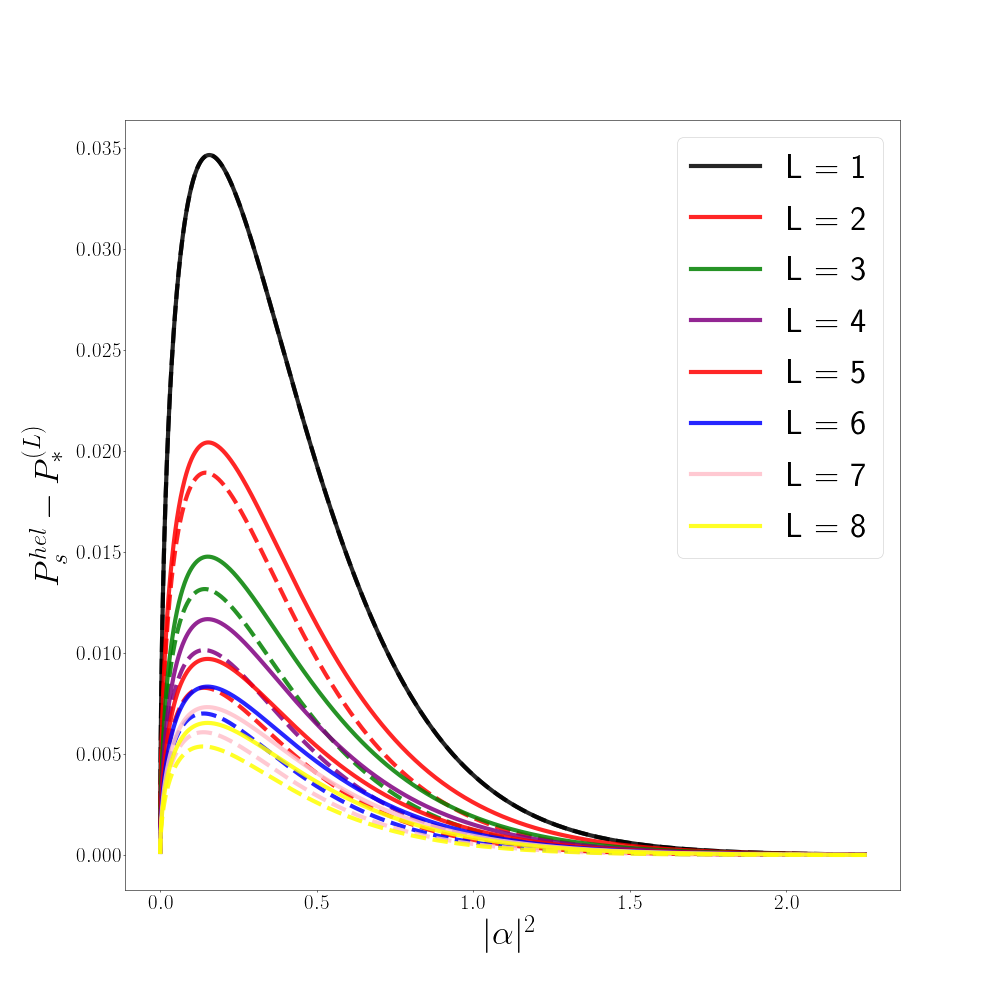
\includegraphics[width=1.\textwidth]{Figures/314/paper_dp_results_notation.png}
        \caption{}
        \label{fig:dpre2}
    \end{subfigure}
    \caption{We show the difference between the best probability of success attainable for a fix $L$ and the optimal probability of success in discriminating BPSK coherent states. The results were obtained by dynamic programming. \textit{Left panel}: the attenuations at the beam-splitters are fixed in such a way that each partial measurement deals with a state having the same intensity $\alpha^{\ell}_k=\frac{\alpha_k}{\sqrt{L-1}}$ for all $\ell$. \textit{Right panel}: we compare the advantage of adapting beam-splitter transmisivities (dashed lines) as compared to the receivers considered in left panel (solid lines).}
    \label{fig:dp_resu}
\end{figure}

Since in the model-aware scenario the agent has full access to the outcomes probabilities, it is sensible to define agent's state as the prior probability of $\ket{\alpha_k}$ at each layer of the receiver. Intuitively, such a quantity stands for the belief distribution over the states $\ket{\alpha_k}$, and it is defined as:
\begin{align}\label{eq:belief}
b_{\ell}(k) = p(\alpha^{(k)}_{\ell}|o_{\ell},a_{\ell-1},b_{\ell-1}).
\end{align}
As new information about the hidden state is collected, the belief evolves. The evolution law of this quantity is obtained by a bayesian update, which reads:
\begin{eqnarray}\label{eq:belUp}
b_{\ell}(k) = \frac{p(\alpha^{(k)}_{\ell}|o_{\ell}, a_{\ell-1}) \;b_{\ell-1}(k)}{\sum_{k} p(\alpha^{(k)}_{\ell}|o_{\ell}, a_{\ell-1}) \; b_{\ell-1}(k)}.
\end{eqnarray}
We can readily define the state value function $v(s)$, recalling it quantifies how \textit{valuable} state $s$ is in terms of the expected return. In our case, the return reduces to the final reward obtained after action $a_L$, \textit{e.g.} guessing, and the expected return becomes the success probability associated to agent's policy. Specifically, agent's policy consists on specifying the actions of its $L$-Dolinar receiver, and we are thus interested in finidng the optimal policy, which on the one hand is linked to Eq.~\ref{eq:32OptSuc}, and on the other hand its state value function should satisfy the optimal Bellman equation.% (\textit{e.g.} Eq.~\ref{eq:vBellOp}).

To understand this last point, let us consider final last step of an $L$-Dolinar receiver, which consists on performing a guess. The optimal action to take is the maximum-likelihood guess, and its associated value function reads
\begin{equation}\label{eq:opBellLQSD}
v^{*}_{L}(b_{L})= \max_{k} b_{L}(k).
\end{equation}
Observe that since $\sum_k b_\ell(k)=1$, it is sufficient to track $b_\ell(k=0)$. The optimal Bellman equation at step $\ell<L$ instead reads
\begin{equation}\label{eq:opBellEllQSD}
v^{*}_{\ell}(b_{\ell})=\underset{a\in\mathcal{A}(s_{\ell})}{\text{max }} \sum_{o_{\ell+1}\in\mathcal{O}} \sum_k p(o_{\ell+1}; b_\ell(k), a_\ell)v^{*}_{\ell+1}(b_{\ell+1}).
\end{equation}
% \begin{equation}\label{eq:opBellEllQSD}
% v^{*}_{\ell}(b_{\ell})=\underset{a\in\mathcal{A}(s_{\ell})}{\text{max }} \sum_{o_{\ell+1}\in\mathcal{O}} \sum_k p(o_{\ell+1}|\alpha_k,a_\ell) b_{\ell}(k)v^{*}_{\ell+1}(b_{\ell+1}).
% \end{equation}

%
% Hence, by computing optimal state-value functions in a recurrent and backward fashion, we are able to find optimal actions for $L$-Dolinar receivers. Specifically, we depart from the final layer ($\ell = L$), and compute the state-value function for a discrete amount (but sufficiently many) of belief values. Note that because of the symmetries highlited in Sec.~\ref{ssec:3bis_intuition}, we can restrict to the interval $\mathcal{B} = \left[0,\frac{1}{2}\right]$, which essentially stands for agent's state space $\mathcal{S}$ of this problem.
The last equation shows that the value-functions can be computed \textit{back-wards}. In this sense, we can first compute the optimal state-value functions for the final layer, then move the previous layer (\textit{i.e.} $\ell = L-1$), and compute optimal ones using Eq.~\eqref{eq:opBellEllQSD} for each belief value in a (discretized) set of possible beliefs $\mathcal{B}$. Because of the symmetry highlighted in Eq.~\ref{eq:symmetry_kenn}, we can consider points in between the interval $[0,\frac{1}{2}]$.

However, we note that for a given $b_\ell \in \mathcal{B}$, the posterior probability $b_{\ell+1}$ appearing in optimal Bellman equation might lie outside the set $\mathcal{B}$. This constitutes a problem, since its state value function is unavailable from the previous step. To circumvent this issue, we interpolate $v_{\ell+1}^*(b)$ to the entire interval $[0,1]$ using Eq.~\ref{eq:symmetry_kenn}, and to this end we require many points in $\mathcal{B}$ (in our numerics we considered $100$).

% Moreover, note that the success of this procedure hinges on the fact that the \textit{optimal} value function was computed, and thus assumes the actions can be optimized correctly. Nevertheless, such optimization can find difficulties. For instance, values of the belief that are close to the extremal points (\textit{e.g.} $0$ or $1$), the optimization landscape flattens, since the success probability already approaches to $1$, and each layer can only contribute with a very small percentage to increase the success probability. Note that such small contributions are actually important, since Dolinar-like receivers assymptotically approach to the Helstrom bound, and thus optimizing such points becomes crucial for large values of $L$. On the other hand, the optimization landscape can present difficulties in the presence of noise, a situation we will discuss below.

% \begin{figure}[b!]
%     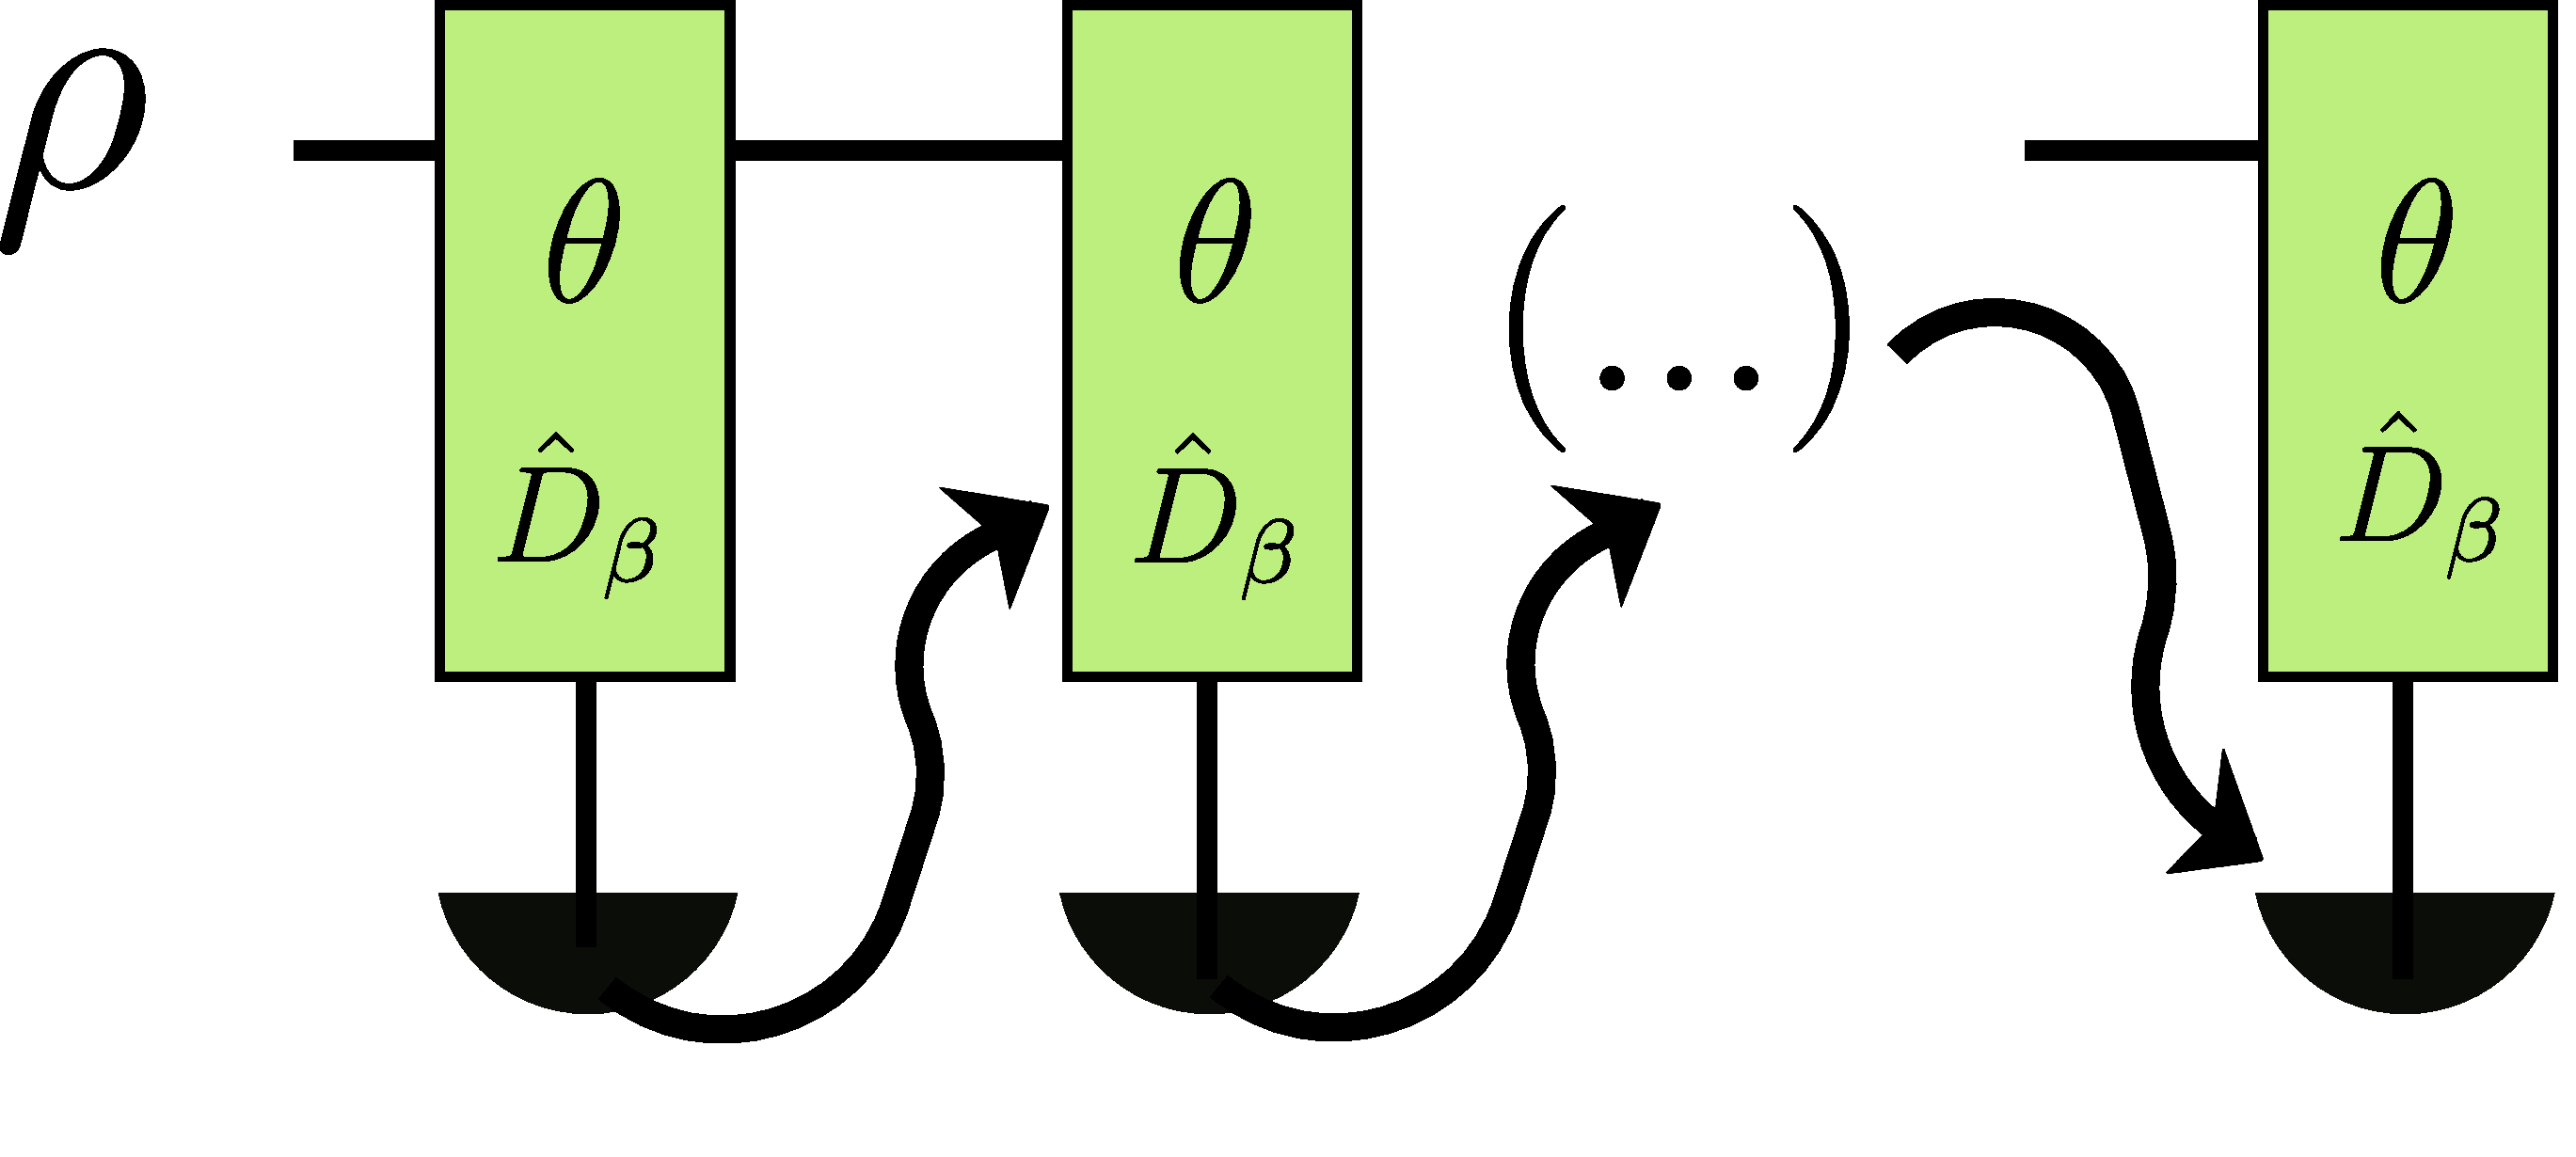
\includegraphics[width=.45\textwidth]{Figures/314/dolinar_receiver_with_theras_adaptive.pdf}
%     \caption{We show an enhanced Dolinar-like receiver, where Beam-Splitter transmisivity values are also conditioned on previous measurement outcome}
%     \label{fig:dolinar_with_attas}
% \end{figure}

In our numerics, shown in Fig.~\ref{fig:dp_resu} we were able to optimize up to $L=30$; the interpolation method is based on Radial Basis Functions (see \textit{e.g.} introduction of Ref.~\cite{rbf_interpolate}) and the minimization method used was dual annealing~\cite{scipy}. Moreover, following a similar proccedure than outlined above, we can optimize over the attenuations as well. The latter proves advantageous, since from $L=4$ and on, adaptive beam-splitters outperform non-adaptive ones, even in the case where an extra layer is included for the latter. To see this, consider Fig.~\ref{fig:dp_resu}: we observe that dashed lines (adaptive beam-splitters) for $L=5$ outperform solid ones (non-adaptive beam-splitters) even for $L=6$.
% As previously pointed out, making use of noisy quantum devices is a tricky task. Here, in order to mitigate the effects of noise, one needs to optimize each possible component of the apparatus. When it comes to Dolinar receivers, there is an additional degree of freedom we have not exploited yet, which is related to the way that the incoming signal is splitted. In particular, the success probability also depends on Beam-Splitters' attenuations, and we could in principle optimize them as well. Thus, we could think on a scheme as the one depicted in Fig.~\ref{fig:dolinar_with_attas}, where the measurement outcome not only conditiones the displacement value, but also the transmissivity of the next BS, which acts on the remaining part of the signal. While conditioning the displacement value according to the measurement outcome can be carried out relatively fast~\cite{Becerra2013,Cook2007}, it is unclear whether we have the technology required to condition transmisivities in a fast way. Nevertheless, we have carried out these numerics which indicate that,

\subsubsection{Unveiling Dolinar's strategy from the numerics}
\begin{figure}[t!]
    \centering
    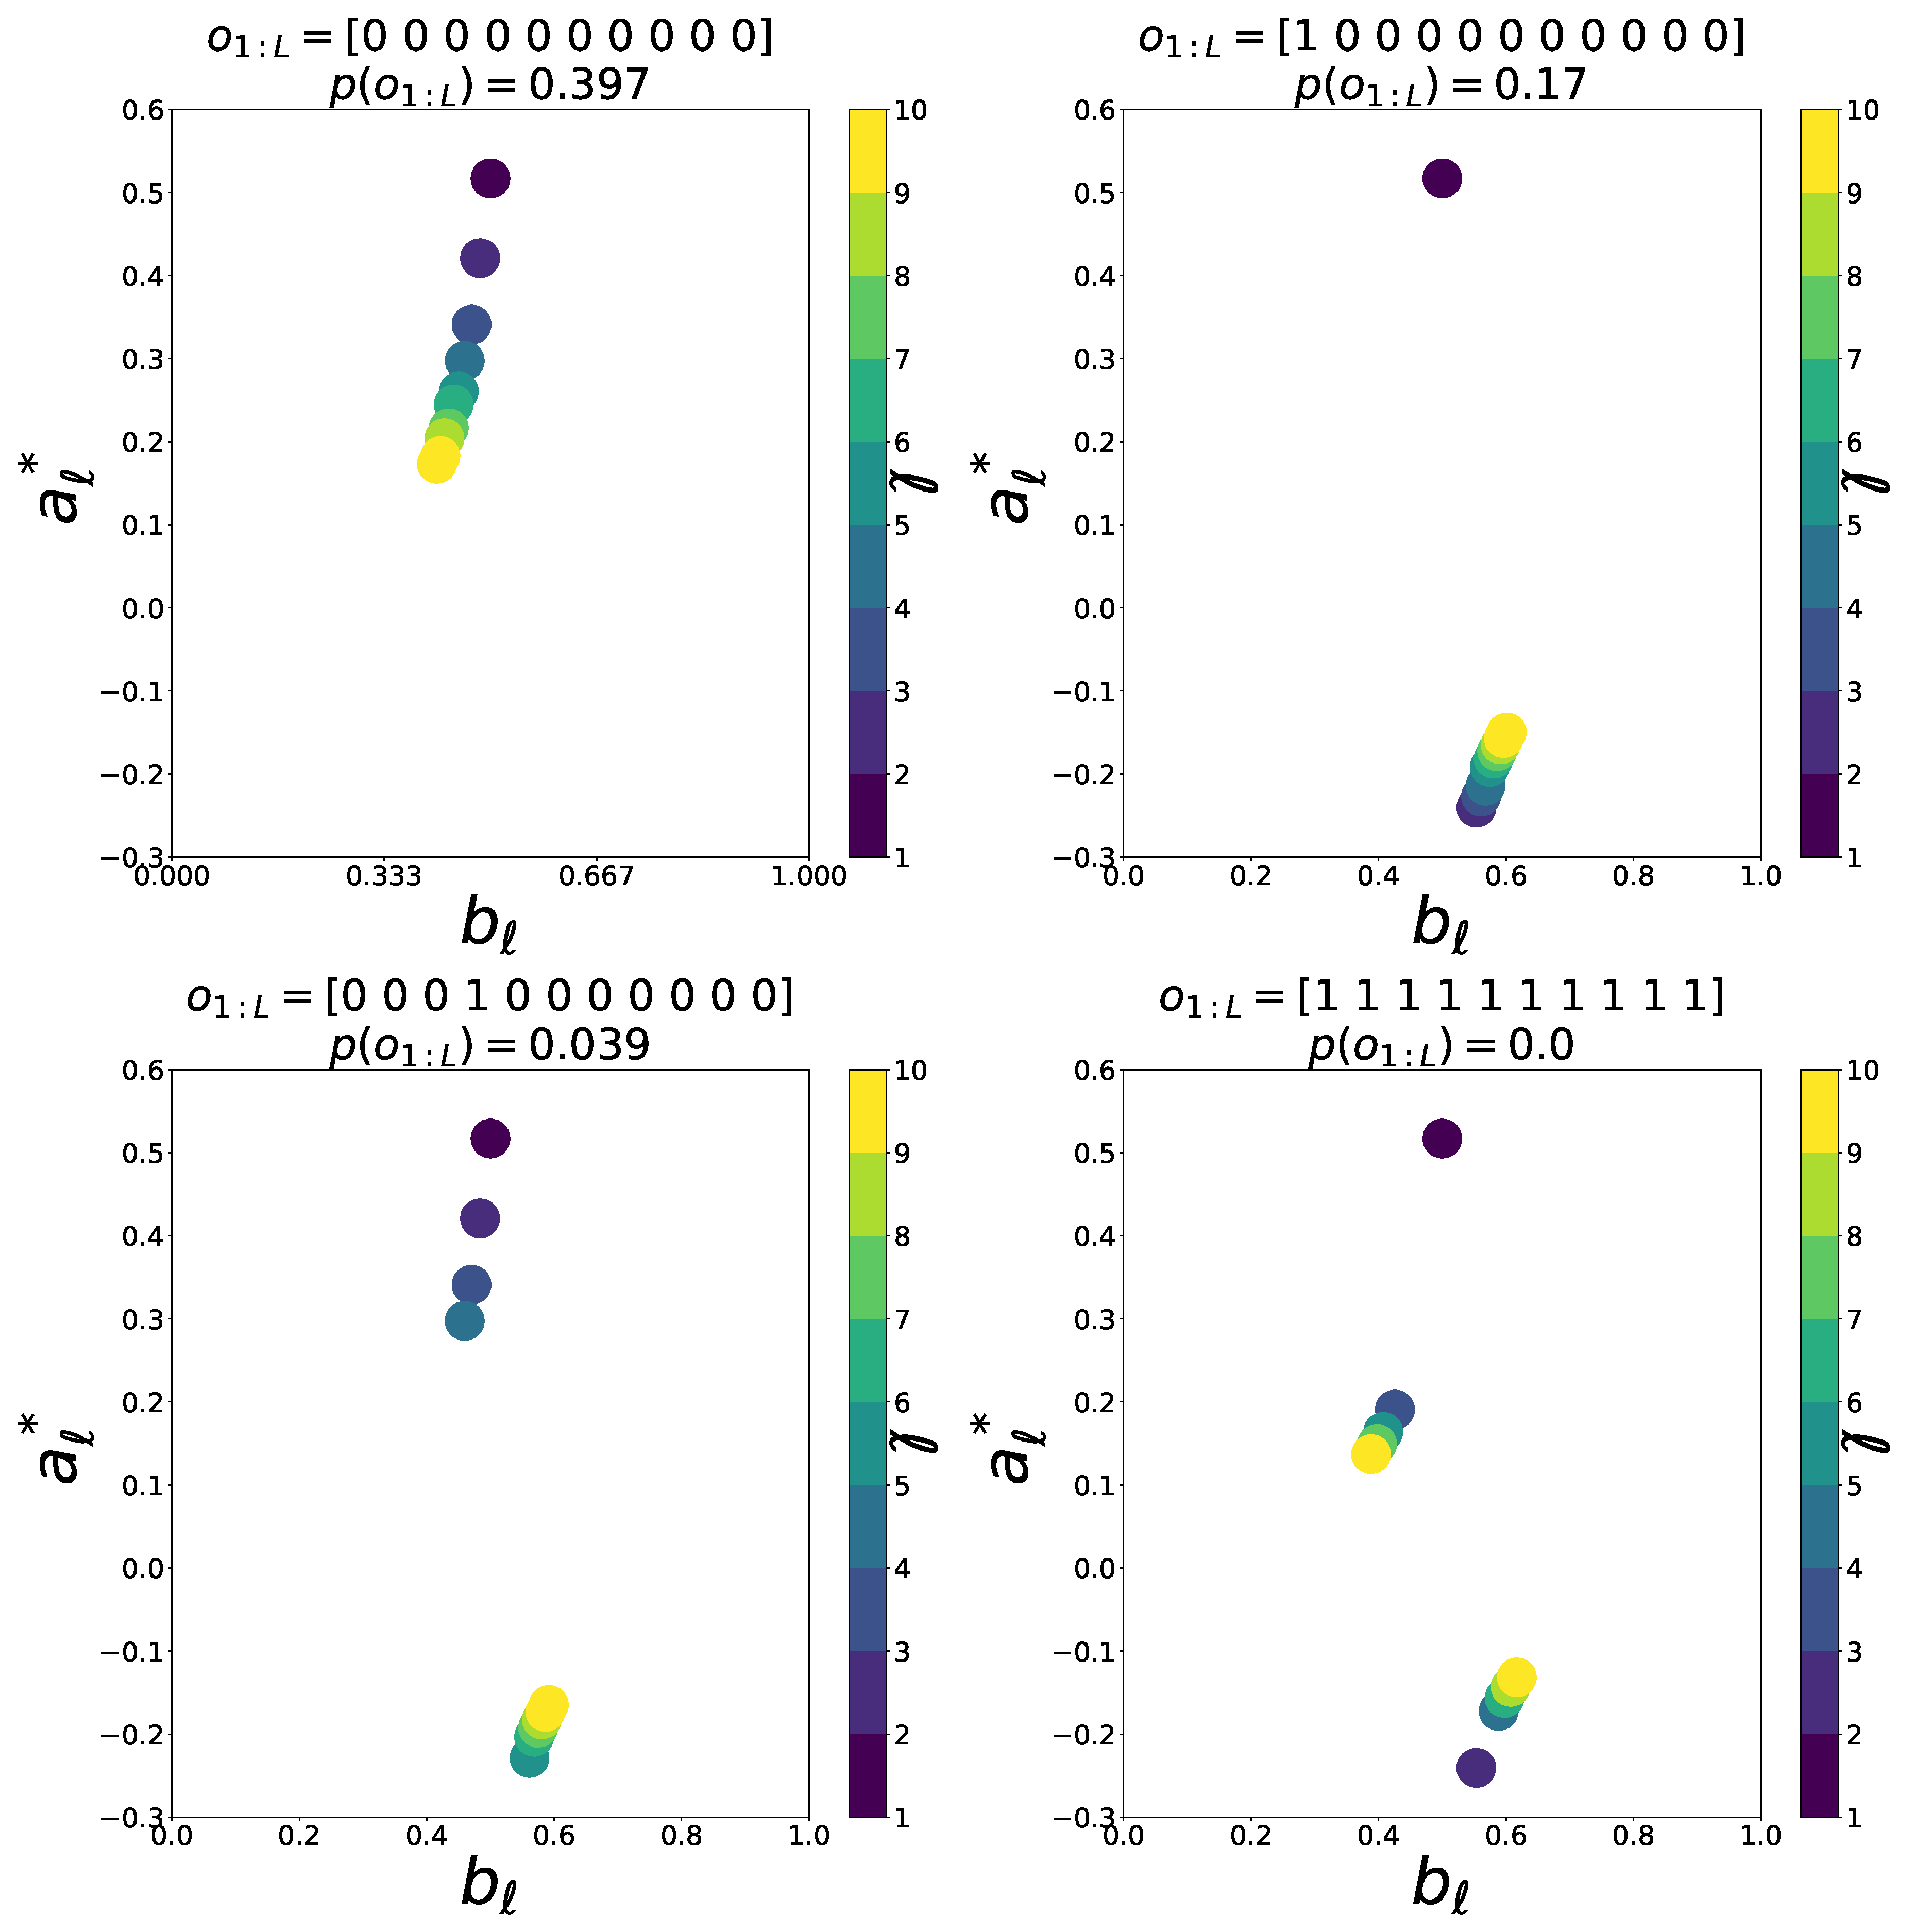
\includegraphics[width=1.\textwidth]{Figures/strat_dolinar.pdf}
    \caption{\small{We show the structure of the optimal policy for a $10$-Dolinar receiver, where we consider $\alpha=0.4$. Each panel corresponds to a different string of observations obtained through a possible experiment realisation. At each layer, the optimal policy obtained through dynamic programming instructs the agent to perform an action (a displacement) according to the current belief $b_\ell$ on state $\ket{\alpha}$; such belief is updated as more information about the environment state is acquired. Thus, in order to obtain this plot, we propagate the initial prior (set to $\frac{1}{2}$) as per Eq.~\ref{eq:belUp}, using the corresponding measurement outcome. Then, we find the interpolate the optimal action that corresponding to that belief, and repeat this along the $10$ layers. Here, we do also compute the total probability of finding each sequence, as per $p(o_{1:L}) = \sum_k p(o_{1:L}|\alpha_k)\eta_k$. Such probability is extremely low for the rightmost sequence (all ones), here rounded to zero, and considerably high for the sequence of all zero outcomes (see discussion in the main body).}}
    \label{fig:strategy_dp}
\end{figure}
\afterpage{\clearpage}

It is worth discussing the optimal strategy, \textit{i.e.} which are the displacements obtained of each layer after the dynamic programming optimization for a fixed $L$. In Fig.~\ref{fig:strategy_dp} we illustrate this optimal strategy, for the $10$-Dolinar receiver. Here, we do only consider a subset of the $2^{10}$ possible combinations of measurement outcomes that can be observed in a single discrimination experiment.

As with Kennedy receiver, Dolinar one is equipped with on/off photodetectors, which projects the incoming state either into the vacuum $\proj{0}$ (no photons), or into its complement $\mathbb{I} - \proj{0}$ (one or more photons). Displacing the signal by $\beta$ right before such measurement acts as a projection $\proj{\beta}$ (or $\mathbb{I}-\proj{\beta}$), and as outlined in Sec.~\ref{ssec:rlcoh_kennedyreceiver} there is a symbiosis between displacements and photon-detection that surpasses the so-called \textit{homodyne limit}, when optimizing over $\beta$.
While for Kennedy receivers $\beta = \alpha$, leading to measure either $\ket{0}$ or $\ket{2 \alpha}$, optimized Kennedy receivers find a better balance between the two contributions by displcing the signal with differnet value (see Fig.~\ref{fig:kenn_compa1}). However, the bottom line is similar: after displacing by a value $\beta>0$ and measuring, if outcome $0$ was obtained, a bet for $\ket{-\alpha}$ is done, and if outcome $1$ is obtained, $\ket{\alpha}$ is then the most likely hypothesis for which the agent bets.

Dolinar receiver exploits this idea, and carries out partial tests in a sequential way. By splitting the signal into $L$ parts, the receiver essentially has now $L$ copies of the state, each attenuated by a factor $\sqrt{L}$. Thus, until a click is detected (measurement outcome $1$), it proceeds similarly to the Kennedy receiver, \textit{i.e.} by testing if the state was $\ket{-\alpha}$. In this sense, the belief of having such state increases according to the number of $0$'s, as can be seen in the Fig.~\ref{fig:strategy_dp}. We also observe that there is a dependence on the value of $\beta$ with the layer number $\ell$, whereas its sign remains positive. However, if the first measurement result happens to be $1$, the preferred hypothesis flips to $\ket{\alpha}$, since by having performed a positive displacement, that is the most-likely state. From there, Dolinar receiver verifies if such claim holds, by testing on the remaining layers whether the state was $\ket{\alpha}$: this is done by changing the sign of the displacement. In turn, if the state $\ket{\alpha}$
was displaced by a value $\beta<0$, then it is more likely to detect outcome $0$. As we can observe in the Figure, if further outcomes happen to be $0$, then the receiver keeps testing $\ket{\alpha}$ through negative displacements. On the contrary, if outcome $1$ is obtained, the strategy flips again (bottom-left panel). The success of Dolinar receiver hinges on the fact that having sequences containing so many consecutive $1$'s is vanishingly small. In turn, for $\alpha=0.4$, we observe that the probability of encountering such a string of outcomes is as small as $10^{-16}$.

We remark that a similar reasoning for the structure of the optimal controls applies in the time-domain Dolinar receiver (see Sec.~\ref{ssec:tdol}), as discussed in Refs.~\cite{Dolinar, Takeoka2005, revisiting2011Assalini}.

We are now in position to turn agnostic, and introduce our reinforcement-learning agent that adapts the receiver to the measurement outcomes sampled from an unknown probability distribution. In such situation, the agent has no other choice than interacting with the receiver through several repetitions of the discrimination experiment, and thus the methods outlined in this Section cannot be applied.
